\documentclass[a4paper, fontsize=11pt]{scrartcl} % A4 paper and 11pt font 
\usepackage[a4paper,left=3cm,right=2cm,top=2.5cm,bottom=2.5cm]{geometry}

\usepackage[T1]{fontenc} % Use 8-bit encoding that has 256 glyphs
\usepackage{fourier} % Use the Adobe Utopia font for the document - comment this line to return to the LaTeX default
\usepackage[spanish]{babel} % Spanish language/hyphenation
\selectlanguage{spanish}
\usepackage[utf8]{inputenc}
\usepackage{amsmath,amsfonts,amsthm} % Math packages
\usepackage{graphicx} % The graphicx package
\usepackage{placeins}
\usepackage{caption}
\usepackage{subcaption}


\usepackage{listings} % Insert Scripts
\usepackage{color} %red, green, blue, yellow, cyan, magenta, black, white
\definecolor{mygreen}{RGB}{28,172,0} % color values Red, Green, Blue
\definecolor{mylilas}{RGB}{170,55,241}

\lstset{language=Matlab,%
	%basicstyle=\color{red},
	breaklines=true,%
	morekeywords={matlab2tikz},
	keywordstyle=\color{blue},%
	morekeywords=[2]{1}, keywordstyle=[2]{\color{black}},
	identifierstyle=\color{black},%
	stringstyle=\color{mylilas},
	commentstyle=\color{mygreen},%
	showstringspaces=false,%without this there will be a symbol in the places where there is a space
	numbers=left,%
	numberstyle={\tiny \color{black}},% size of the numbers
	numbersep=9pt, % this defines how far the numbers are from the text
	emph=[1]{for,end,break},emphstyle=[1]\color{red}, %some words to emphasise
	%emph=[2]{word1,word2}, emphstyle=[2]{style},    
}

\usepackage{sectsty} % Allows customizing section commands
%\allsectionsfont{\centering \normalfont\scshape} % Make all sections centered, the default font and small caps

\usepackage{fancyhdr} % Custom headers and footers
\pagestyle{fancyplain} % Makes all pages in the document conform to the custom headers and footers
\fancyhead{} % No page header - if you want one, create it in the same way as the footers below
\fancyfoot[L]{} % Empty left footer
\fancyfoot[C]{} % Empty center footer
\fancyfoot[R]{\thepage} % Page numbering for right footer
\renewcommand{\headrulewidth}{0pt} % Remove header underlines
\renewcommand{\footrulewidth}{0pt} % Remove footer underlines
\setlength{\headheight}{13.6pt} % Customize the height of the header

\numberwithin{equation}{section} % Number equations within sections (i.e. 1.1, 1.2, 2.1, 2.2 instead of 1, 2, 3, 4)
\numberwithin{figure}{section} % Number figures within sections (i.e. 1.1, 1.2, 2.1, 2.2 instead of 1, 2, 3, 4)
\numberwithin{table}{section} % Number tables within sections (i.e. 1.1, 1.2, 2.1, 2.2 instead of 1, 2, 3, 4)

%\setlength\parindent{0pt} % Removes all indentation from paragraphs - comment this line for an assignment with lots of text

\newenvironment{myalign}{\par\nobreak\large\noindent\align}{\endalign} %Altering fontsize in equations globally

%----------------------------------------------------------------------------------------
%	TITLE SECTION
%----------------------------------------------------------------------------------------

\newcommand{\horrule}[1]{\rule{\linewidth}{#1}} % Create horizontal rule command with 1 argument of height

\title{	
	\normalfont \normalsize 
	\textsc{Master en Automática y Robótica - UPM} \\ [25pt] % Your university, school and/or department name(s)
	\horrule{0.5pt} \\[0.4cm] % Thin top horizontal rule
	\huge Control por Realimentación del Estado \\ % The assignment title
	\horrule{2pt} \\[0.5cm] % Thick bottom horizontal rule
}

\author{Jorge Camarero Vera - 07052} % Your name

\date{\normalsize\today} % Today's date or a custom date

\begin{document}
	\maketitle
	
	\section{Explicación de la tarea}
	
	La finalidad de esta tarea es obtener el modelo en el espacio de estados de la función de transferencia (\ref{TransferFunction}) en forma canónica  controlable discreta.
	
	\begin{myalign}
		G(s) = \dfrac{1}{(s+1)(s+2)(s+5)}
		\label{TransferFunction}
	\end{myalign}
	
	Para conseguir el sistema controlable se deberán situar los polos en:
	
	\begin{myalign}
		\begin{split}
			&p1 = -10\\
			&p2 = -1+i\\
			&p3 = -1-i\\
		\end{split}
	\label{Poles}
	\end{myalign}
	
	\subsection{Desarrollo de la tarea}
	
	Calculamos el modelo en el espacio de estados en forma canónica continua de la siguiente forma:
	
	\begin{lstlisting}
	num = [1];
	den = poly([1 2 5]);
	[A B C D] = tf2ss(num, den);
	sys = ss(A,B,C,D)
	
	sys =
	
	a = 
	     x1   x2   x3
	x1    8  -17   10
	x2    1    0    0
	x3    0    1    0
	
	b = 
	    u1
	x1   1
	x2   0
	x3   0
	
	c = 
	    x1  x2  x3
	y1   0   0   1
	
	d = 
	    u1
	y1   0
	
	Continuous-time state-space model.
	\end{lstlisting}
	
	Se emplea la función \textit{tf2ss} para convertir la función de transferencia (\ref{TransferFunction}) en el espacio de estados. Y la función \textit{ss} para organizar las matrices del espacio de estados en un objeto de \textit{Matlab} para manejar más fácilmente modelos en el espacio de Estados.\\
	
	Vemos que el modelo se encuentra en una \textbf{forma canónica continua} del espacio de estados. Ahora veremos si el modelo es controlable de la siguiente forma:
	
	\begin{lstlisting}
	CtrbMatrix = ctrb(sys);
	Controllability = rank(CtrbMatrix)
	
	Controllability =
	
	3
	\end{lstlisting}
	
	Vemos que el rango de la matriz de controlabilidad es máximo, por tanto el sistema es controlable.\\
	
	El sistema es controlable, pero de momento la salida ante escalón unitario es inestable, tiende a infinito, Figura \ref{Conitunous Output 0}.
	
	\begin{figure}[h!]
		\centering
		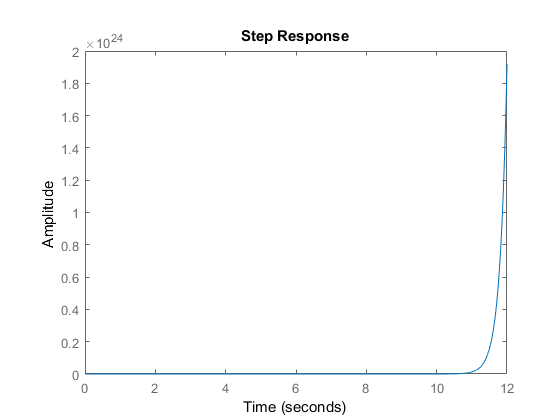
\includegraphics[width=1.0\linewidth]{images/StepOutput0.png}
		\caption{Salida continua del sistema no controlado ante entrada escalón unitario.}
		\label{Conitunous Output 0}
	\end{figure}
	\FloatBarrier
	
	Para obtener el sistema controlable debemos calcular la matriz de realimentación para situar los polos del modelo en el lugar de los polos dados en (\ref{Poles}). Para ello se ha utilizado la función \textit{place}, de la siguiente manera y conseguimos el modelo controlable en la forma continua:\\
	
	\begin{lstlisting}
	K = place(sys.a, sys.b, [-10 -1+i -1-i])
	
	K =
	
	20.0000    5.0000   30.0000
	
	sys_cl = ss(sys.a - sys.b*K, sys.b, sys.c, sys.d)
	
	sys_cl =
	
	a = 
 	     x1   x2   x3
	x1  -12  -22  -20
	x2    1    0    0
	x3    0    1    0
	
	b = 
	    u1
	x1   1
	x2   0
	x3   0
	
	c = 
	    x1  x2  x3
	y1   0   0   1
	
	d = 
	    u1
	y1   0
	
	Continuous-time state-space model.
	\end{lstlisting}
	
	
	Se obtiene una salida, Figura \ref{Conitunous Output}, en este modelo ante una entrada escalón unitario.\\
	
	\begin{figure}[h!]
		\centering
		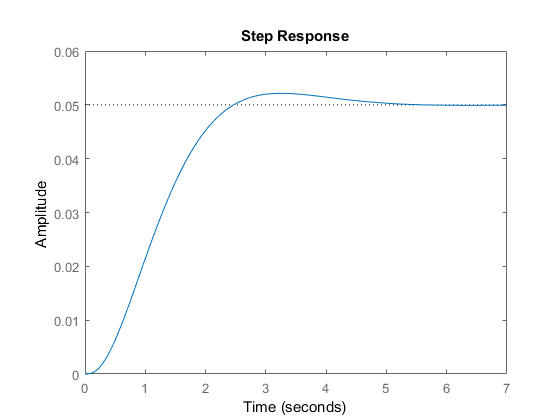
\includegraphics[width=1.0\linewidth]{images/StepOutput.png}
		\caption{Salida continua del sistema controlado ante entrada escalón unitario.}
		\label{Conitunous Output}
	\end{figure}
	\FloatBarrier
	
	Para obtener el modelo discreto empleamos la función \textit{c2d} empleando un tiempo de muestreo de $T_s = 0.1$ segundos.\\
	
	\begin{lstlisting}
	Ts = 0.1;
	
	sys_cl_d = c2d(sys_cl, Ts)
	
	sys_cl_d =
	
	a = 
	          x1        x2        x3
	x1    0.2488    -1.303    -1.122
	x2   0.05612    0.9222  -0.06843
	x3  0.003421   0.09718    0.9975
	
	b = 
	           u1
	x1    0.05612
	x2   0.003421
	x3  0.0001254
	
	c = 
	    x1  x2  x3
	y1   0   0   1
	
	d = 
	    u1
	y1   0
	
	Sample time: 0.1 seconds
	Discrete-time state-space model.
	\end{lstlisting}
	
	Y como el sistema no está en forma canónica la transformamos:
	
	\begin{lstlisting}
	sys_canon_d = canon(sys_cl_d, 'companion')
	
	sys_canon_d =
	
	a = 
	        x1      x2      x3
	x1       0       0  0.3012
	x2       1       0  -1.481
	x3       0       1   2.169
	
	b = 
	    u1
	x1   1
	x2   0
	x3   0
	
	c = 
	           x1         x2         x3
	y1  0.0001254  0.0006495   0.001292
	
	d = 
	    u1
	y1   0
	
	Sample time: 0.1 seconds
	Discrete-time state-space model.
	
	step(sys_canon_d)
	\end{lstlisting}
	
	Obteniéndose la salida ante entrada escalón unitario, Figura \ref{Discrete Output};
	
	\begin{figure}[h!]
		\centering
		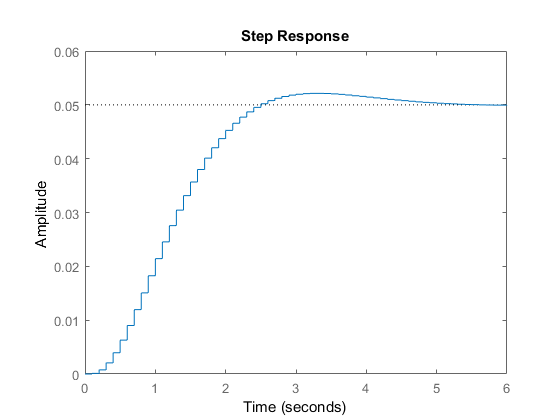
\includegraphics[width=1.0\linewidth]{images/StepOutput2.png}
		\caption{Salida discreta del sistema controlado ante entrada escalón unitario.}
		\label{Discrete Output}
	\end{figure}
	\FloatBarrier
	
	Comparando la salida del sistema continuo y el discreto, Figura \ref{Compared Output}, vemos que para el muestreo se ha empleado un \textbf{bloqueador de orden 0}.
	
	\begin{figure}[h!]
		\centering
		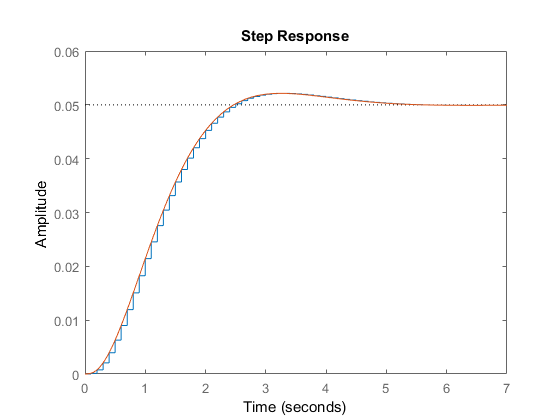
\includegraphics[width=1.0\linewidth]{images/ComparedOutput.png}
		\caption{Salida discreta y continua del sistema controlado ante entrada escalón unitario.}
		\label{Compared Output}
	\end{figure}
	\FloatBarrier
	
\end{document}